\documentclass[a4paper,12pt]{report}
\usepackage[utf8]{inputenc}
\usepackage{amsmath}
\usepackage{graphicx}
\usepackage{listings}
\usepackage{tikz}
\usepackage[T1]{fontenc}
\usepackage{color}
\usetikzlibrary{arrows,automata}
\definecolor{pythonred}{rgb}{0.6,0,0} % for strings
\definecolor{pythongreen}{rgb}{0.25,0.5,0.35} % comments
\definecolor{pythonpurple}{rgb}{0.5,0,0.35} % keywords
	\definecolor{pythondocblue}{rgb}{0.25,0.35,0.75} % javadoc
	 
	\lstset{language=python,
	basicstyle=\ttfamily,
	keywordstyle=\color{pythonpurple}\bfseries,
	stringstyle=\color{pythonred},
	commentstyle=\color{pythongreen},
	morecomment=[s][\color{pythondocblue}]{/**}{*/},
	numbers=left,
	numberstyle=\tiny\color{black},
        stepnumber=2,
	numbersep=10pt,
	tabsize=4,
	showspaces=false,
	showstringspaces=false}

% Title Page

 \title{\bfseries\huge \textcolor{purple}{\underline {EEP-703 Computer Network Lab}} \\{\textcolor{blue}{Assignment3-Client-Server stubs in C/C++ in UNIX environment}}}
\author{\bfseries\large\textcolor{black}  {Harshit Kumar Gupta}\\ {\textcolor{black} {2013EET2369 }}\\

\includegraphics[width=3cm,height=3.4cm]{./iit.png}\\\noindent Computer Technology\\
\noindent Department Of Electrical Engineering\\IIT DELHI}
% iit.png: 282x282 pixel, 72dpi, 9.95x9.95 cm, bb=0 0 282 282
\begin{document}
\maketitle
\tableofcontents


\chapter{\textcolor{blue}{\underline {PROBLEM STATEMENT}}}
\noindent 
         Basics of Network Programming: An introduction to the basics of writing client-server stubs in C/C++ in UNIX
environment.\\\\
\begin{enumerate}
 \item Problem Statement (a)
  Using C-C++ develop a client­server scenario in which server acts as a data provider to clients.
The server holds a student directory which contains Name, Entry Number and Email ID for each
student. A client can request for a student’s email ID by providing either his-her name or entry
number. In response server should return the corresponding student record (all fields). Use TCP
sockets and a text file for database which has been mailed to the group.
\item Problem Statement (b)
Implement a query based system as follows:
RETURN <year>
(e.g. RETURN 2012 should return records of all students with entry in
2012)
RETURN *
(return all records)
ADD <name> <entry no> <email id>
(e.g. add a new student record for given arguments)
\item Problem Statement (c)
Upgrade your server code to serve multiple clients simultaneously. Please note that server must
be able to handle several write requests at the same time.
\end{enumerate}

 



\begin{center}
\chapter{\textcolor{blue}{\underline {ABSTRACT}}}
\end{center}
\noindent The Intention of the C Code is to make use of Socket Programming to create a Server and a Socket Client on a TCP approach
	  where we are supposed to send the Search string from the Client side and send it to the Server.
	  The Server then in return send backs the entire record for that student and displays it on the Client terminal.

\begin{center}
\chapter{\textcolor{blue}{\underline {INTRODUCTION}}}
\end{center}
\noindent  In all computer networks, one of the computers acts as a server (for applications, data, services)
to client computers. In this assignment, we will learn how to develop the C/C++ code which is
used to program this functionality on the client and on the server.\\\\
	  C is one of the most widely used programming languages of all time, and C compilers are available for the majority of available computer architectures and operating systems.
, C has facilities for structured programming and allows lexical variable scope and recursion, while a static type system prevents many unintended operations. Its design provides constructs that map efficiently to typical machine instructions,
and therefore it has found lasting use in applications that had formerly been coded in assembly language, most notably system software like the Unix computer operating system.
	  
\begin{center}
\chapter{\textcolor{blue}{\underline {SPECIFICATIONS AND ASSUMPTIONS}}}
\end{center}
\section*{Specifications}
\begin{enumerate}
 
\item bind() function has been used to bind the hostaddress
\item buffer size used is 256 as it is sufficient.
\item The input file database.txt is stored in the same path.
\item Socket Programming has been implemented in C language.
\end{enumerate}

\section*{Assumptions}
\begin{enumerate}
\item There are as such no multiple entries for the same student.
\item The search String accept character Values only.
\item Error handling has been done accordingly for non existent records or as such.
\end{enumerate}
 
\begin{center}
\chapter{\textcolor{blue}{\underline {LOGIC USED/METHODOLOGY}}}
\end{center}
The methodology that is used for developing this project work is defined below:
\begin{enumerate} 
\item First of all a Server is To be Created and the port no is defined.
\item The Server Code also connects to the Database File where Records are Saved.
\item A buffer is defined so as to save the Input file.
\item Now the Socket function is called and structure Intialised.
\item Host address is bind using the bind() call.
\item Now the input Search string say name is sent to the server.
\item Server searches for the String match and returns the Corresponding Record value.
\item If the User eneters some Invalid value , the error message is displayed.
\end{enumerate}

\begin{center}
\chapter{\textcolor{blue}{\underline {FLOWCHART}}}
\end{center}
\noindent Flowchart\\
\begin{center}
 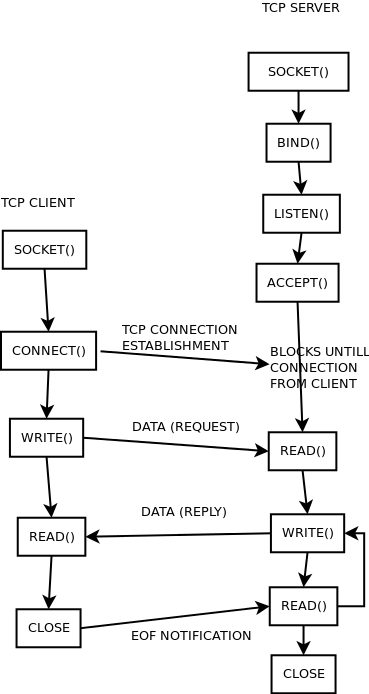
\includegraphics[width=12 cm,height=12 cm]{./flowchart.png}
 % flowchart.png: 351x439 pixel, 96dpi, 9.29x11.61 cm, bb=0 0 263 329
\end{center}

\begin{center}
\chapter{\textcolor{blue}{\underline {Execution Directives}}}
\end{center}
\noindent \\ In the terminal of LINUX system the following commands are executed in order to create a network topology and its analysis.\\
\begin{enumerate}
  \item Simply Compile the file writing gcc -o QueryServer server.c service.c -lpthread
  \item Set the Server host to telnet <hostaddress> <Portno>
  \item Ensure that there exists a file named database.txt
  \item Now simply run the file using ./QueryServer Command
  \item Pass the Commands to the Telnet Client-
\\name <NAME> 
\\entry <ENTRYNO>
\\return *
\\return <YEAR>
\\add <NAME> <ENTRYNO> <EMAILID
\\quit
\end{enumerate}



\begin{center}
\chapter{\textcolor{blue}{\underline {RESULTS AND CONCLUSIONS}}}
\noindent We find that for the given search values the code seems to work perfectly fine and returns the value exactly as the 
	  record of that student which is supposed to be accessed.
 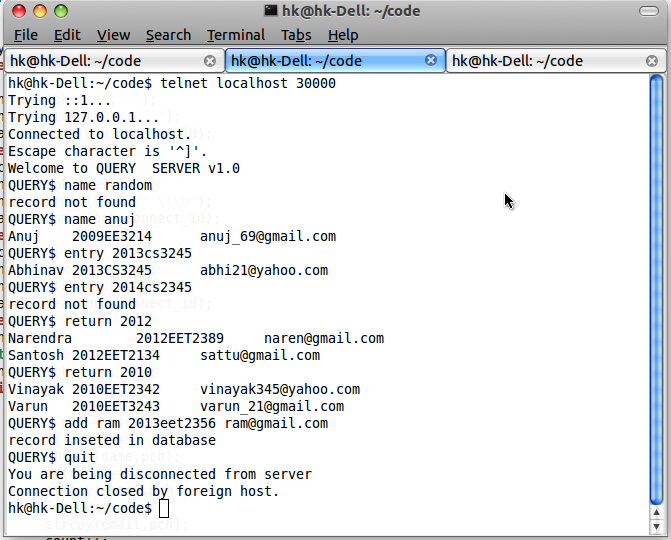
\includegraphics[width=12 cm,height=12 cm]{./Screenshot.png}
 % flowchart.png: 351x439 pixel, 96dpi, 9.29x11.61 cm, bb=0 0 263 329
\end{center}


\end{document}  